\par Durant notre stage de fin d’études, nous avons eu la chance de travailler au sein d’une équipe opérationnelle et bien organisée, dont les membres sont dotés de l’esprit d’équipe, d’entre-aide et du sens d’initiative et de créativité.
\par Dans la présente Section, on va découvrir ces équipes là et les projets aux quel j'ai eu la chance de contribuer.

\begingroup
\let\clearpage\relax
\chapter{OST/ITS/INV/MDM}
\endgroup

\par Comme toutes les grandes multinationales, Amundi AM recense un nombre incalculable de départements, de secteurs ou d'équipes. Dans le chapitre suivant, je vais décrire l’organisation générale des deux équipes où j’ai effectué mon stage, en suivant une approche descendante.
\\~\\

\section{OST: Operations Services \& Technologies}

\par Amundi AM est subdivisée en plusieurs entités principales (nommée Divisions), on retrouve notamment les départements administrant le groupe Amundi AM (par exemple le département DGL, présidé par Mr. Perrier Yves, président et directeur général du groupe Amundi), les départements relatifs au relations clients Amundi AM (par exemple INS: Institutional Clients Division, RET: Retail Clients Division \dots). Ensuite on retrouve les divisions responsables des activités d'Amundi AM, a savoir BSC (Business Support \& Control) et OST (Operations services \& Technologies). 
\par Présidé par Mr. Lesage Guillaume, cette division regroupe les différents départements essentiels a la gestions d'actifs, activité principale d'Amundi AM. On retrouve par exemple le service NEG (Negociation), ASM (Asset Servicing Management), ASV (Amundi Services) et AFN (Amundi Finance). En plus de ces départements, la division contient aussi ITS (Amundi Technology, IT Services), département auquel j'ai été affecté, qui contient à son tour plusieurs services. 
\clearpage
\section{ITS: Amundi Technology, IT Services}

\begin{figure}[ht]
    \centering
    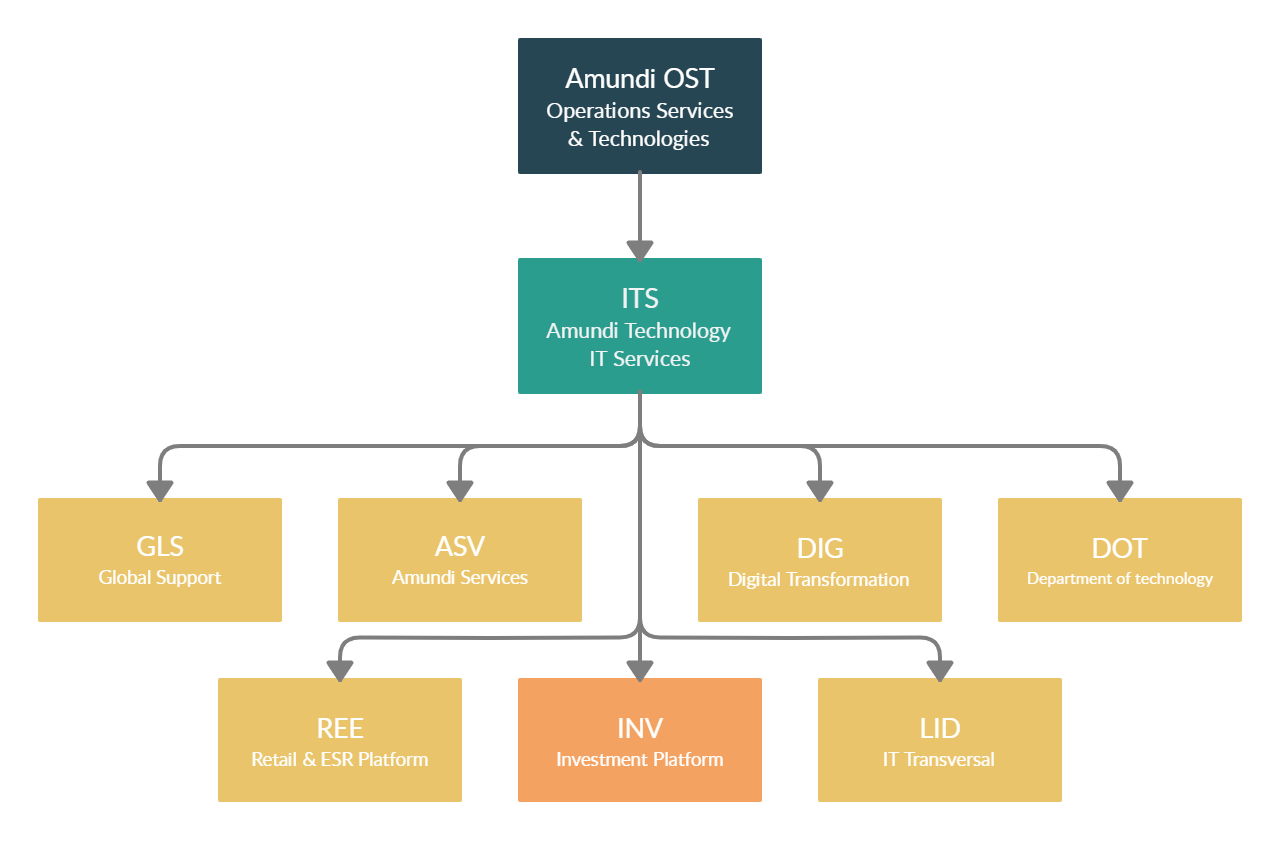
\includegraphics[width=\columnwidth]{img/Org ITS.png}
    \caption{Organisation ITS}
    \label{fig:its}
\end{figure}

\par Le département ITS, comme le nom l'indique, est le département responsable de tout ce qui est service IT. Il est composé de sept services comme le montre la figure \ref{fig:its} ci-dessus: 
\begin{itemize}
    \item GLS (Global Support): la branche d'Amundi ITS basé à Dublin (Irlande) subdivisée en deux services, DHB (Dublin Hub and Intl. Development)\& DOT (Department of technology: Dublin Hub and infrastructure)
    \item ASV (Amundi Services): Amundi services (cf. Part I. Chapitre II.)
    \item DIG (Digital Transformation): Service mutualisé avec le département BSC (Business support and control) chargé de la transformation et communication digitale.
    \item DOT (Department of technology): regroupe les équipes qui travaillent sur le côté hardware (architecture, infrastructure et réseaux), Frameworks internes (dont un que j'ai eu la chance d'utiliser dans un projet) et gestion de base de données. 
    \item REE (Retail \& ESR Platform): Service gérant deux applications Amundi AM majeurs, Alto Retail et ESR. 
    \item LID (IT Transversal): Leading IT Department
    \item INV (Investment Management Platform): Service qui est subdivisé en plusieurs équipes, responsables de plusieurs applications client et interne Amundi AM. Service auquel j'ai été affecté et qu'on va détailler dans la prochaine section
\end{itemize}

\section{INV: Investment Management Platform}
\par Comme c'est déjà mentionné dans la précédente section, le service INV est subdivisé en plusieurs équipes (comme le montre la figure \ref{fig:inv} ci-dessous).\\
\begin{itemize}
    \item EAX: Entreprise Architecture \& UX Design, Equipe qui ce charge de tout ce qui design et maquettes d'applications (User Interface, User Experience) (Notamment utilisé dans le projet Alto Investment Research cf. XXXX) 
    \item FOA: Front Office \& Analysis, Equipe qui se charge des projets Front office (cf. Partie I. Chapitre II. Section I. Sous-Section "Organisation d'un Asset Manager")
    \item RIS: Risk Development
    \item DHB: Dublin Hub Development, précédemment cité dans la Section 2 du Chapitre I. de la partie II. est l'equipe INV basée a Dublin (Irlande). Elle se compose principalement du projet PKC (Position Keeping \& Control) XXXX
    \item INS: Institutional XXXX
    \item TTP: Trading \& MO Trade Processing XXXX
    \item MDM: Master Data Management, Equipe a laquelle je suis affecté, la prochaine section de ce chapitre essayera de détailler ses missions, applications gérés, et périmètre de fonctions.
\end{itemize}
\par Chaque équipe gère des applications essentiels au activités d'Amundi AM.
\begin{figure}[ht]
    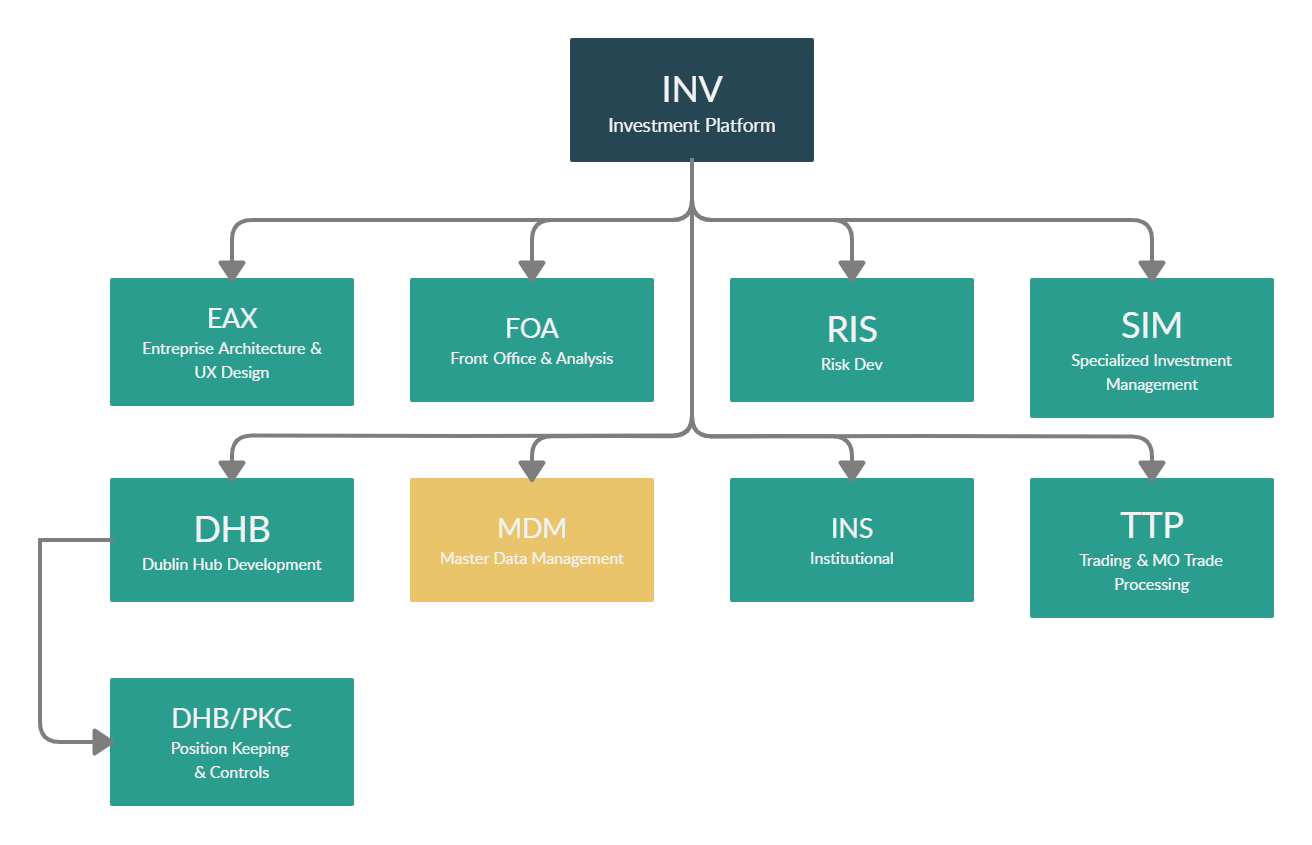
\includegraphics[width=\columnwidth]{img/Org INV.png}
    \caption{Organisation INV}
    \label{fig:inv}
\end{figure}

\section{MDM: Master Data management}


% Atlas
% BIFI
% DQC
% EWR
% FundLife
% Hubref
% Libra
% Life
% MDBM
% MDQC
% Medco
% OpenAml
% Refgt
% Refms
% rgp